%==================================================================================================
%   LUKES THESIS TEMPLATE 1.2
%   -------------------------
%   This template is based upon the offcial IMM PhD Thesis template, it is enhanced with a number
%   of new features and a number of errors have fixed. This template is intended to be complied to
%   PDF using PDFLATEX and is tested using the MiKTeX 2.9 LaTeX distribution.
%   It is based on the official DTU-IMM Thesis template by Finn Kuno Christensen in 2009.
%   Small bugfixes by Kasper Laursen in 2012 and 2013.
%   Small updates by Finn Kuno Christensen/Henning Christiansen in 2015.
%   -------------------------
%   Last Updated: 2015-01-08
%==================================================================================================
%
%==================================================================================================
% DOCUMENT SETUP
%==================================================================================================
\documentclass[10pt,twoside]{book}                  %Official DTU-IMM Thesis document setup
%
%Set to 'print' for printed version, use 'net' for online version
\def\thesisversion{print}
%
%==================================================================================================
% PACKAGES
%==================================================================================================
\usepackage{LukeThesis}                             %Import Thesis base style
\usepackage{wrapfig}
\usepackage{pdfpages}
\usepackage{lscape}
%input{PhDMacros}                                   %Thesis specific macros
%
\usepackage{mwe}
\usepackage{listings}    
\usepackage{etoolbox}
\usepackage{booktabs}
\usepackage{url}
\usepackage{hyperref}
\usepackage{graphicx}
\usepackage{subfig}


%%Listings settings
\definecolor{mygreen}{rgb}{0,0.7,0}
\definecolor{mygray}{rgb}{0.47,0.47,0.33}
\definecolor{myorange}{rgb}{0.8,0.4,0}
\definecolor{mywhite}{rgb}{0.98,0.98,0.98}
\definecolor{myblue}{rgb}{0.01,0.61,0.98}
\definecolor{myclearblue}{rgb}{0.04,0.55,0.98}
\definecolor{bluekeywords}{rgb}{0.13,0.13,1}
\definecolor{greencomments}{rgb}{0,0.5,0}
\definecolor{redstrings}{rgb}{0.9,0,0}

\newcommand*{\FormatDigit}[1]{\ttfamily\textcolor{black}{#1}}
%% http://tex.stackexchange.com/questions/32174/listings-package-how-can-i-format-all-numbers


\lstdefinestyle{FormattedNumber}{%
	literate=*{0}{{\FormatDigit{0}}}{1}%
	{1}{{\FormatDigit{1}}}{1}%
	{2}{{\FormatDigit{2}}}{1}%
	{3}{{\FormatDigit{3}}}{1}%
	{4}{{\FormatDigit{4}}}{1}%
	{5}{{\FormatDigit{5}}}{1}%
	{6}{{\FormatDigit{6}}}{1}%
	{7}{{\FormatDigit{7}}}{1}%
	{8}{{\FormatDigit{8}}}{1}%
	{9}{{\FormatDigit{9}}}{1}%
	{.0}{{\FormatDigit{.0}}}{2}% Following is to ensure that only periods
	{.1}{{\FormatDigit{.1}}}{2}% followed by a digit are changed.
	{.2}{{\FormatDigit{.2}}}{2}%
	{.3}{{\FormatDigit{.3}}}{2}%
	{.4}{{\FormatDigit{.4}}}{2}%
	{.5}{{\FormatDigit{.5}}}{2}%
	{.6}{{\FormatDigit{.6}}}{2}%
	{.7}{{\FormatDigit{.7}}}{2}%
	{.8}{{\FormatDigit{.8}}}{2}%
	{.9}{{\FormatDigit{.9}}}{2}%
	%{,}{{\FormatDigit{,}}{1}% depends if you want the "," in color
	{\ }{{ }}{1}% handle the space
	,%
}


\lstset{%
	backgroundcolor=\color{mywhite},   
	basicstyle=\footnotesize,       
	breakatwhitespace=false,         
	breaklines=true,                 
	captionpos=b,                   
	commentstyle=\color{mygray}, 
	deletekeywords={...},           
	escapeinside={\%*}{*)},          
	extendedchars=true,              
	frame=shadowbox,                    
	keepspaces=true,                 
	keywordstyle=\color{myorange}, 
	keywordstyle=[2]\color{mygreen},    
	language=Octave,                
	morekeywords={*,...},            
	numbers=left,                    
	numbersep=5pt,                   
	numberstyle=\tiny\color{mygray}, 
	rulecolor=\color{black},         
	rulesepcolor=\color{myblue},
	showspaces=false,                
	showstringspaces=false,          
	showtabs=false,                  
	stepnumber=2,                    
	stringstyle=\color{blue},    
	tabsize=2,                       
	title=\lstname,
	emphstyle=\color{myclearblue},%  style for emph={} 
}    

%% language specific settings:

\lstdefinestyle{sharpc}{language=[Sharp]C, frame=lr, rulecolor=\color{blue!80!black}}


\lstdefinestyle{Processing}{%
	style=FormattedNumber,
	keywords={int, float, boolean, PVector, color, Integer, String},
	keywords=[2]{setup, draw, if, else, else if. return, for, true, false, new},%               define keywords
	morecomment=[l]{//},%             treat // as comments
	morecomment=[s]{/*}{*/},%         define /* ... */
	emph={import, radians, void, size, this, println, exit, stroke, strokeWeight, background, smooth, translate, rotateX, rotateY, scale, beginShape, point, endShape, length, vertex, fill, text, toString, get, mult, add, line, pushMatrix, translate, applyMatrix, popMatrix, sub, set, cross, normalize, sqrt, sq, atan2, sin, cos, null, equals, substring, parseInt},%        keywords to emphasize
}


\lstdefinestyle{Arduino}{%
	style=FormattedNumber,
	keywords={print, Servo, begin, analogRead, Serial, map, delay, attach, available, readStringUntil, substring, length, toCharArray, write, atoi, println, equals},
	keywords=[2]{while, if, else, else if, setup, loop, while, return},%               define keywords
	morecomment=[l]{//},%             treat // as comments
	morecomment=[s]{/*}{*/},%         define /* ... */
	emph={const, int, void, String},%        keywords to emphasize
}

\lstdefinestyle{WWWClass}{%
	style=FormattedNumber,
	keywords={var, function, yield},
	keywords=[2]{while, if, else, else if, setup, loop, while, return},%               define keywords
	morecomment=[l]{//},%             treat // as comments
	morecomment=[s]{/*}{*/},%         define /* ... */
	emph={new, Renderer},%        keywords to emphasize
}

\newtoggle{InString}{}% Keep track of if we are within a string
\togglefalse{InString}% Assume not initally in string
%==================================================================================================
% THESIS PROPERTIES (Modifiy these fields with your details)
%==================================================================================================
\def\thesisauthor{Adrian Llopart Maurin (P.h.D.)}                     %Author
\def\thesistitle{RBPF-SLAM in \textit{MatLab} \\ Users Guide}               %Title
\def\thesishandin{05-May}                       %Submission date (Day-Month}
\def\thesisdegree{P.h.D.}                              %Degree ('B.Eng', 'B.Sc.', 'M.Sc.' or 'PhD')
\def\thesisyear{2016}                               %Submission year
\def\thesisnumber{}                             %DTU-IMM Serial number (do not include year)
\def\thesisISSN{}                          %ISSN number
\def\thesiskeywords{}  %PDF keywords
\derivethesisprops                                  %Derive dependent properties
%
%==================================================================================================
% SECTION NUMBERING SETUP
%==================================================================================================
\setcounter{tocdepth}{2}                            %2 adds sections up to subsections
\setcounter{secnumdepth}{3}                         %Subsubsections get a number when this is 3
%
%==================================================================================================
% THESIS STRUCTURE  (Modifiy to include more chapters etc)
%==================================================================================================
\begin{document}
%------------------------
%Pre-frontmatter material
%------------------------
\prefrontmatter
%--------------------
%Frontmatter material
%--------------------
\frontmatter
\pagenumbering{roman}                               %Set frontmatter numbering style
\chapter{Abstract}
Rao-Blackwellized Particle filters have been introduced in simultaneous localization and mapping (SLAM) effectively in the past years. Improved techniques have helped reduce the number of particles needed and allowed a faster and more robust solution. These solutions can be seen, and used, in the C++ ROS \textit{gmapping} package. This manual presents the conversion to a simpler but easy-to-understand \textit{MatLab} implementation and will describe the RBPF-SLAM principle in a similar manner.   
\label{Abstract}                                %English summary of Thesis
\markboth{}{}                                       %Set headings (left)(right)
                        

%------------------
% Table of contents
%------------------
\newpage\mbox{}\newpage
\chaptermark{Contents}
\pdfbookmark{\contentsname}{toc}
\renewcommand{\sectionmark}[1]{\markright{#1}}
\sectionmark{Contents}
\addtolength{\parskip}{-\baselineskip}
\tableofcontents
\addtolength{\parskip}{\baselineskip}
\renewcommand{\sectionmark}[1]{\markright{\thesection\ #1}}
%-------------
% Main content
%-------------
\mainmatter
\chapter{Introduction}
One of the clearest functionalities of mobile robots is building maps of its surroundings and navigating through them; this is often referred to as SLAM, Simultaneous Localization and Mapping. There exists, however, certain difficulties when implementing SLAM, mainly, for a robot to localize (know its true position), a very precise map has to be built before; but, for a very precise map to be built, a robot must know exactly where it is. Friction, control loss or small obstacles are often the cause of a bad odometry which leads to a poor estimate of the true position. The Rao-Blackwellized Particle filter (as shown in ~\cite{Doucet} and ~\cite{Murphy}) solves this issue by generating estimates of the possible position (particles) and giving them a weight. Those particles that have a higher weight, because their estimate matches better the reality, will survive, and the rest will die out in the next generation. To keep a continuous amount of particles and not let all of them die out, resampling stages are carried out where those surviving particles reproduce and keep the particle count constant. It is evident that the more particles used, the more possible descriptions of the reality one has and the higher probability of having at least one particle which is almost perfect. This also induces a higher computational necessity and stops the solution from becoming a real-time application.\\
The real issue is, therefore, weighing these particles to know how close they are to the reality. This is known as the \textit{proposal distribution} $\pi$, and in the latter iterations of the RBPF-SLAM solution, optimal techniques have been developed to obtain a more accurate representation, whilst keeping the particle count to a minimum.\\
In summary, what the RBPF-SLAM algorithm does is given an initial estimate of the true pose, it will use the high precision of a laser scan and the latest map generation to converge the estimate to the true position. This leads to a more accurate map representation and a considerable reduction in errors and number of particles.
\section{MapGeneration}
\subsection{Introduction}
In a real-world application of the RBPF-SLAM, the real odometry and laser scans of a robot would be used. For a simulation, however, these values need to be generated by the user. To do so, a simulation map will be created, and a simulated robot will move through it following a determined path. Laser scan data will be derived mathematically and will be fed, together with a error-incorporated odometry, into the RBPF-SLAM method, that will generate different particles and maps to better adjust to the reality of the simulation.

\subsection{Creating the map}
The construction of the map is done through individual walls. A matrix \textit{map} (with dimensions 4xn) will represent these walls. The first row corresponds to the x-coordinate of the initial point of the wall; and the second row will be the y-coordinate. Similarly, the third and fourth row are the x and y coordinates of the final wall point, respectively. 

\begin{equation}
	map(:,n) = [x_{initial}; y_{initial}; x_{final}; y_{final}];
\end{equation}

Therefore the user can create whichever map he/she feels fit, as complex or simple as wanted. the result can be visualized uncommenting the next few lines of code.

\subsection{Path generation}

Once the map is complete, the path the robot will follow has to be detailed. This is done in the \textit{via} vector which incorporates the coordinates of points in the path the robot has to travel through. The \textit{MatLab} function \textit{mstraj} by Peter Corke uses the defined \textit{via}, maximum axis-speed limits and a timestep to determine the trajectory (\textit{path}) of the robot.

\subsection{Control parameters}
\label{Errors}
This is precisely where the control aspect of robotics comes into place. A controller has to be developed to make the robot follow the path as desired. in other words, you will pre-program the robot to follow a certain path instead of giving it movement commands at every time step. The parameters that have to be tuned are $d$, $K_p$ and $K_h$. The error signals in the feedback control loop are calculated as follows:

The absolute distance from the desired position (in \textit{path}) and the latest position $x_{t-1}(x,y,\theta)$ given by the latest movement control command $u_{t-1}$: 
\begin{equation}
	e = \sqrt{((path_{1, t}-x_{1, t-1})^2 + (path_{2, t}-x_{2, t-1})^2)} - d;
\end{equation}
The angular error between these two positions:
\begin{equation}
	th = atan2((path_{2, t}-x_{2, t-1}),(path_{1, t}-x_{1, t-1}));
\end{equation}

The new movement control commands will be:
\begin{equation}
	u_{1, t} = K_p \cdot e;
\end{equation}
\begin{equation}
	u_{2, t} = K_h \cdot (angdiff(th,x_{3, t-1}));
\end{equation}

The resulting path after tunning the controller can be visualized commenting out the RBPF line (\textbf{[pf.xh(:,k),pf] = RBPF(x(:,k),y,LRS,u(:,k-1),a,pf, Nsamples,'multinomial\_resampling')}) and uncommenting the true position plotting section that follows it.



\section{MotionModel}
\subsection{Introduction}
\textit{Motion models} comprise the state transition probability $p(x_t|u_t. x_{t-1})$ to determine a new position given its previous one and the movement control command. Therefore, theprobailistic kinematic approach will be used (instead of a deterministic one) because it takes into consideration the control uncertainty due to noise or unmodelled exogeneous effects.\\
Since many commercial mobile robots are actuated by independent translational and rotational velocities, a \textit{velocity motion model} will be used, as presented in \cite{ProbabilisticRobotics}.

\subsection{Motion error parameters}
This motion model relies on the robot specific motion error parameters $\alpha_1$ to $\alpha_6$. The values of these parameters have to be calculated for each robot specifically. The resulting odometry distribution will vary in great amounts because of them. Translational error is given by $\alpha_1$ and $\alpha_2$, the angular error by $\alpha_3$ and $\alpha_4$, and $\alpha_5$ and $\alpha_6$ represent the end rotation error.\\
The method \textit{Motion\_Model\_Velocity\_Test} allows for a fast, simple and visually-appealing calculation of these values. Given a starting position ($x_{t-1}$), a movement command ($u_{t}$) and a grid size $[x_g, y_g ]$, it will generate the odometry proposal distribution as seen in the following figures:

\begin{figure}[h]
	\centering
	\begin{minipage}{.48\textwidth}
		\renewcommand\figurename{Fig.}
		\centering
		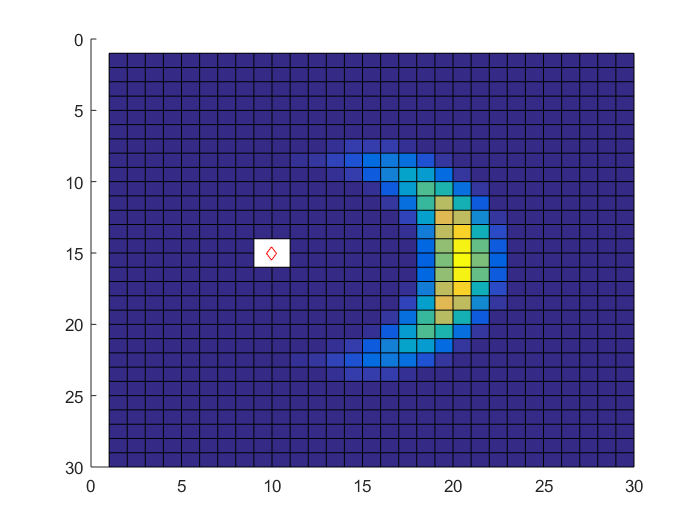
\includegraphics[width=0.95\linewidth]{figures/MotionModel_1}
		\caption{Odometry distribution for a $u_t$=[10 0] and an $a$=[0.01 0.01 0.01 0.1 0.001 0.001]}
	\end{minipage}%
	\hfill
	\begin{minipage}{.48\textwidth}
		\renewcommand\figurename{Fig.}
		\centering
		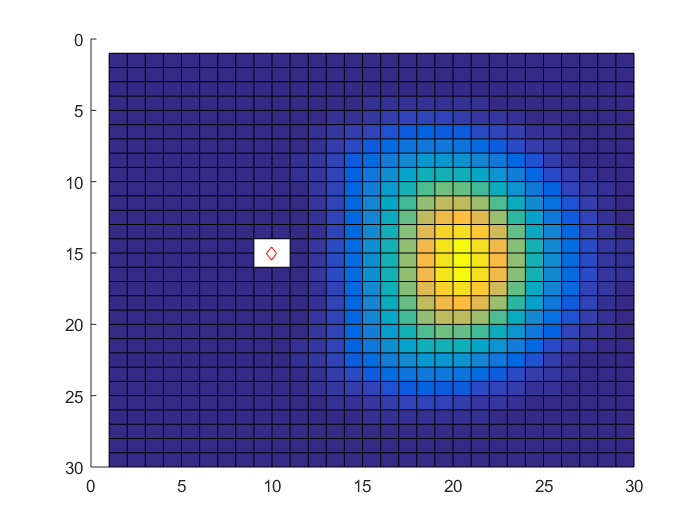
\includegraphics[width=0.95\linewidth]{figures/MotionModel_2}
		\caption{Odometry distribution for a $u_t$=[10 0] and an $a$=[0.1 0.1 0.01 0.01 0.001 0.001]}
	\end{minipage}%	
\end{figure}

It is suggested that you evaluate how big your movement commands $u_t$ are for every time step (they are dependant on the number of points \textit{path} has) adn the \textit{maximum velocity} set in the \textit{mstraj} function. Once you have an estimate, use the \textit{Motion\_Model\_Velocity\_Test} to see how your odometry distribution would look like for different motion error parameters $\alpha$. Try to fine-tune these values so that the simulated odometry error resembles the reality.


\section{RBPF-SLAM}
Once the map has been correctly generated and the simulated robot follows an adequate trajectory, it is time to enable the Rao-Blackwellized Particle Filter.\\
In the \textit{Simulation parameters} section at the top of the \textit{Main} code one can modify many parameters that have a direct impact on the result of the RBPF:

\begin{itemize}
	\item \textit{Ts}: Sampling time, by default set to happen every second.
	\item \textit{n\_cell}: sets how many centimetres a cell represents. The default is that each cell has an area of 10$cm^2$. The modification of this value should not change the structure of the code nor give any errors, but this has not been tested out yet so it is \textbf{not guaranteed} to work.
	\item \textit{NPC}: Number of particles. The more particles selected, the more accurate the occupancy grid will become, but the more computational power required for the calculations. The main advantage of the improved techniques used in this simulator for RBPF-SLAM is that the total amount of particles can be kept very low (3-6) and the results will still be fairly accurate to the reality.
	\item \textit{usable\_area}: When running the particle filter, only data in a radius of \textit{usable\_area} will be utilized, specifically, the occupancy map and the laser scan data. 
	\item \textit{sigma\_v}: Describes the standard variation of the sensor beam.
	\item R1: represents the variance matrix for the odometry. Small changes in the variance have great effects on the filter.
	\item \textit{Nsamples}: Corresponds to the number of samples to be taken when creating the Gaussian distribution. 
	\item \textit{max\_speed}: The maximum speed of the simulated robot in the vertical and horizontal axis, taking into account the size of each cell.
	\item \textit{LRS\_Sensor structure parameters}: to be set according to the laser scanner you want to model.
	\item \textit{L}: The occupancy grid is initialized to have a value of 0.5 in all of its cells. This will change on every iteration of the filter, updating the cell value to describe the probability of an exiting wall in that location.
\end{itemize}

\subsection{Filter initialisation}
The first time step of the simulation will be an initialisation of the occupancy grid map. Since we have not moved yet, the position estimate corresponds to the true value. Therefore, the generated map at this point will be very similar to the reality (except for minor laser scan variances). For this reason, the map is updated with the first scan and the particle weights and locations (which in both cases are the same for all particles) are initialised.

\subsection{RBPF simulation}
From the second iteration onwards, the particle filter will work continuously updating positions of particles and their maps. At the beginning of every iteration the new movement commands $u_t$ are calculated (based off the \textit{e} and \textit{theta} errors mentioned in section \ref{Errors}). The new true position $x_t$ is calculated assuming no errors (ideal case that does not match the reality) and 'true' scan data is obtained from the simulation.\\
The \textbf{RBPF} function is then triggered, taking all the above as arguments. After various variable initializations, the filter starts working for every particle:\\
An initial estimate of the position $x_t$ is obtained from the previous particle positions $\ddot x_{t-1}$, the movement command $u_t$ and the variance matrix $R1$ (another option would be to sample one time directly from the motion model). An estimated laser scan is obtained from teh estimated position and the last iteration of the occupancy grid map for that particle via the \textbf{Measurement\_Estimate\_From\_Grid} method. Before the ICP (scan-matching) algorithm can be applied, the 'true'scan $y$ and the estimated one $y_h$ have to be pre-processed. Since the laser data is in radial form (laser angle and distance) it will be easier to match one-to-one scan. To do so, all scans that have a distance bigger than \textit{usable\_area} will be depreciated. This helps computational-wise and focuses only on scans that come from areas of the map that are closer to the robot and, thus, are more reliable. Theoretically, those scans that are neglected in $y$ should also be in $y_h$, and vice versa. In reality, sometimes they do not and those scans that mismatch because of this will also be neglected to avoid errors in the ICP algorithm. Finally, the scans are converted to Cartesian space and put in the World frame and the initial estimate position $x_t$ is also included in the point cloud for reasons described below.\\
The ICP algorithm is run between both datasets ($y$ and $y_h$). If the ICP reports a failure or generates translational or rotational matrices which are erroneous, the final position estimate of the particle $\ddot x_t$ will be equal to the initial estimate $x_t$ that simply came from the odometry distribution. In the cases where the ICP succeeds, a translational $TT$ and rotational $TR$ matrix are returned; these represent the movement the estimated laser scan data $y_h$ has to follow to converge to the 'true' scan data $y$. 

\begin{wrapfigure}{L}{0.4\textwidth}
	\renewcommand\figurename{Fig.}
	\begin{center}
		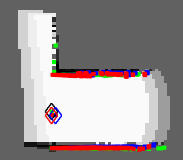
\includegraphics[width=0.38\textwidth]{figures/path-image}
	\end{center}
	\caption{Different position estimates and scans: true, before ICP and after}
\end{wrapfigure}

The trick here is that the ICP also returns the rotated data (which should, in most cases, have converged), and since the initial estimated position was included in the dataset, a better estimate of the position $\dot x_t$ thanks to scan-matching is already derived (the $\theta$ value will remain the same as the one previously estimated). This is automatically visualized through a figure which has, in the background, a grey-scaled image of the occupancy grid map up until that point, the diamond shaped points that represent the positions (black: true position, blue: initial estimate, red: new estimated position after scan-matcher). In the same manner, the laser scans are represented where green is the true scan, blue is the scan obtained from the previous occupancy map and an initial estimate, and red would be the converged scan.

The next step is obtaining samples $x_j$ to create the Gaussian distribution. These samples are randomly selected around $\dot x_t$ and will be used to evaluate the target proposal consisting
of the odometry distribution $p(x_j|x_{t-1}^{(i)}, u_t)$ and the observation likelihood $p(z_t| x_j, m^{(i)})$. The former is derived by means of the function \textbf{Motion\_Model\_Velocity} which returns the probability of a final position given an initial one and a movement command. The latter is obtained via a scan matching procedure. The approach selected is a point-to-point comparison between the true scan and the scan obtained from the current map for that sample. Both distributions are then multiplied point-wise to obtain the target proposal $\tau$.\\
The weighing factor $\eta^{(i)}$, the Gaussian mean $\mu_t^{(i)}$ and the covariance $\Sigma_t^{(i)}$ are calculated. The particle weights are also updated. Additionally, the final position estimate for that particle $\ddot x_t$ is sampled from the Gaussian. Finally, the map for that particle is updated given the final estimated position $\dot x_t$ and the true laser scan.\\
To check if a resample is necessary, the weights are normalized and $N_eff$ is derived. In the case that this value is smaller than a given percentage of the total amount of particles, a resampling step must be taken. If not, no further steps are required.





%-----------
% Backmatter
%-----------
\backmatter
\chaptermark{Bibliography}
\renewcommand{\sectionmark}[1]{\markright{#1}}
\sectionmark{Bibliography}
\addcontentsline{toc}{chapter}{Bibliography}        %Force addition of Bibliography to TOC
\bibliographystyle{abbrv}                           %Use alpha codes for references
\bibliography{References}                           %Bibliography file called
         
\end{document}
% % % EOF % % %